% Attribution : J.-M. Arnaudiès, Problèmes de préparation à l’agrégation de mathématiques, t. 2, problème 42, p. 289 (Ellipses, 1999).
% Source autonome. Compiler deux fois avec pdflatex.
% Les figures sont dessinées en TikZ. Aucun fichier annexe n'est nécessaire.
\documentclass[a4paper,12pt]{article}
\usepackage[T1]{fontenc}
\usepackage[utf8]{inputenc}
\usepackage{lmodern,amsmath,amssymb}
\usepackage[a4paper,left=22mm,right=22mm,top=24mm,bottom=22mm,headheight=14pt,headsep=7mm,footskip=12mm]{geometry}
\usepackage{xcolor,graphicx,tikz,fancyhdr,needspace}
\usepackage[unicode,colorlinks=true,linkcolor=deep,urlcolor=accent,pdfauthor={},pdftitle={Concours d'entrée à l'ENS Ulm, juin 1966. Le problème de Koszul. Sujet et corrigé}]{hyperref}
\definecolor{deep}{HTML}{123D4A}
\definecolor{accent}{HTML}{087777}
\definecolor{wash}{HTML}{EAF4F2}
\definecolor{ink}{HTML}{1A2730}
\definecolor{soft}{HTML}{526871}
\definecolor{clay}{HTML}{AC542E}
\definecolor{peach}{HTML}{FAEADF}
\setlength{\parindent}{0pt}
\setlength{\parskip}{3.7pt plus .5pt minus .5pt}
\setlength{\abovedisplayskip}{7pt plus 2pt minus 2pt}
\setlength{\belowdisplayskip}{7pt plus 2pt minus 2pt}
\setlength{\abovedisplayshortskip}{2pt}
\setlength{\belowdisplayshortskip}{5pt}
\raggedbottom
\emergencystretch=1.6em
\newcommand{\R}{\mathbb R}
\newcommand{\Id}{\mathrm{Id}}
\newcommand{\Om}{\Omega}
\newcommand{\norm}[1]{\lVert #1\rVert}
\newcommand{\ps}[2]{(#1\mid #2)}
\DeclareMathOperator{\rang}{rang}
\DeclareMathOperator{\im}{Im}
\DeclareMathOperator{\tr}{tr}
\newcommand{\rubrique}{REPÈRES}
\pagestyle{fancy}
\fancyhf{}
\fancyhead[L]{\small\sffamily\color{soft}ALGÈBRE LINÉAIRE}
\fancyhead[R]{\small\sffamily\color{soft}SUJET ET CORRIGÉ}
\fancyfoot[L]{\small\sffamily\color{soft}Endomorphismes extrémaux}
\fancyfoot[R]{\small\sffamily\color{soft}\thepage\ / \pageref*{fin}}
\renewcommand{\headrulewidth}{0.3pt}
\newcommand{\partie}[2]{\renewcommand{\rubrique}{PARTIE #1}\phantomsection\pdfbookmark[1]{Partie #1. #2}{part-#1}\label{bloc-#1}%
  {\sffamily\bfseries\large\color{accent}Partie #1\enspace\textcolor{soft}{/}\enspace #2\par}\vspace{1pt}}
\newcounter{pas}
\newsavebox{\boitequestion}
\newcommand{\enonce}[3]{\par
  \setcounter{pas}{0}%
  \sbox{\boitequestion}{\begingroup\setlength{\fboxsep}{6pt}\colorbox{wash}{%
   \parbox{\dimexpr\linewidth-2\fboxsep\relax}{%
   {\small\sffamily\bfseries\color{accent}QUESTION #1\hfill ÉNONCÉ ORIGINAL\par}
   \vspace{2pt}{\raggedright\color{deep}\ignorespaces#3\par}}}\endgroup}%
  \Needspace{\dimexpr\ht\boitequestion+\dp\boitequestion+5\baselineskip\relax}
  \smallskip\pdfbookmark[2]{#1. #2}{q-#1}\noindent\usebox{\boitequestion}\par
  \nobreak{\small\sffamily\bfseries\color{deep}Résolution\par}\nobreak}
\newcommand{\etape}[1]{\par\Needspace{2.25\baselineskip}\smallskip\stepcounter{pas}%
  \textbf{\textcolor{deep}{\thepas.\enspace #1}}\enspace\ignorespaces}
\newcommand{\suite}[1]{\par{\small\sffamily\bfseries\color{accent}#1\par}\smallskip}
\newcommand{\idee}[1]{\etape{Idée.}#1\par}
\newcommand{\bilan}[1]{\par\smallskip\noindent
  \begingroup\setlength{\fboxsep}{6pt}\colorbox{peach}{\parbox{\dimexpr\linewidth-2\fboxsep\relax}{\color{deep}\textbf{Réponse.}\enspace #1}}\endgroup\par\smallskip}
\newcommand{\legende}[1]{{\small\sffamily\color{soft}#1\par}}
\providecommand{\og}{«~}
\providecommand{\fg}{~»}
\begin{document}
\color{ink}

{\sffamily\bfseries\fontsize{22}{25}\selectfont\color{deep}Concours d'entrée à l'ENS Ulm, juin 1966\par}
{\sffamily\color{soft}\href{https://fr.scribd.com/document/603917743/ens-ulm-1966}{Le problème de Koszul}\enspace$\cdot$\enspace Endomorphismes extrémaux d'un cône\par}
\smallskip
{\sffamily\bfseries\small\color{accent}DONNÉES COMMUNES DE L’ÉNONCÉ\par}
On désigne par $E$ un espace vectoriel euclidien de dimension $3$ et on note $\ps{x}{y}$ le produit scalaire de deux vecteurs appartenant à $E$. On désigne par $u$ un vecteur unitaire de $E$ et par $\sigma$ la symétrie qui transforme tout élément $x\in E$ en $\sigma(x)=x-2\ps{x}{u}u$.

Soit $\Omega$ l'ensemble des $x\in E$ tels que $\ps{x}{\sigma(x)}\leq0$ et $\ps{x}{u}\geq0$. On désigne par $N$ l'ensemble des endomorphismes $\alpha$ de $E$ tels que $\alpha(\Omega)\subset\Omega$ et par $N_+$ l'ensemble des endomorphismes de la forme $\beta+\gamma$, où $\beta$ et $\gamma$ sont deux éléments de $N$ linéairement indépendants dans l'espace des endomorphismes de $E$. On dira qu'un endomorphisme de $E$ est \emph{extrémal} s'il appartient à $N$ et n'appartient pas à $N_+$.

\partie{I}{Le cône et les premiers rangs}

\enonce{I.1}{Comment reconnaître un vecteur du cône grâce au produit scalaire ?}{%
Comparer $\Omega$ et l'ensemble des éléments $y\in E$ tels que $\ps{y}{x}\geq0$ pour tout $x\in\Omega$.
}
\etape{Lire les deux conditions qui définissent $\Omega$.}
Concrètement, $E$ est l’espace de nos vecteurs. Trois axes perpendiculaires permettent de les décrire par trois coordonnées, comme dans $\R^3$. Choisissons $u$ pour verticale et notons $e_1,e_2$ deux directions horizontales perpendiculaires de longueur $1$. Dans la base $(e_1,e_2,u)$, on a $u=(0,0,1)$. Un vecteur $x=(a,b,s)$ a pour hauteur $\ps{x}{u}=s$ et pour partie horizontale $v=(a,b,0)$. Ainsi $x=su+v$. La symétrie soustrait deux fois la hauteur, donc $\sigma(x)=(a,b,-s)$. En multipliant les coordonnées correspondantes puis en additionnant, on obtient
\[
 q(x):=\ps{x}{\sigma(x)}=a^2+b^2-s^2=\norm{v}^2-s^2.
\]
La condition $q(x)\leq0$ donne $\norm v\leq |s|$. Comme on demande aussi $s\geq0$, on obtient \textbf{$x\in\Omega$ exactement quand $s\geq\norm v$}. Par exemple, $(3,4,6)$ est à l'intérieur car $6>\sqrt{3^2+4^2}=5$, tandis que $(3,4,5)$ est sur le bord.

\etape{Vérifier qu'un $y$ du cône réussit tous les tests.}
Écrivons $y=ru+w$, avec $w$ horizontal. Pour $x,y\in\Omega$, on a $s\geq\norm v$ et $r\geq\norm w$. Même si les parties horizontales pointent en sens opposés, l'inégalité de Cauchy--Schwarz garantit que $\ps{w}{v}\geq-\norm w\norm v$. Ainsi
\[
                   \ps{y}{x}=rs+\ps{w}{v}\geq rs-\norm w\norm v\geq0 .
\]

\etape{Vérifier la réciproque.}
Supposons $\ps{y}{x}\geq0$ pour tout $x\in\Omega$. En prenant $x=u$, on trouve $r\geq0$. Si $w\ne0$, testons $x=u-w/\norm w$. Sa hauteur est $1$ et sa partie horizontale, de longueur $1$, pointe exactement à l'opposé de $w$. Ce vecteur est sur le bord et donne
\[
                  0\leq\ps{y}{x}=r-\frac{\ps{w}{w}}{\norm w}=r-\norm w .
\]
Donc $r\geq\norm w$, ce qui place $y$ dans le cône. Pour $w=0$, le premier test $r\geq0$ suffit déjà.
\bilan{Les deux ensembles sont égaux. Cette propriété de $\Omega$ s'appelle l'autodualité.}

\enonce{I.2}{Quels sont les extrémaux de rang zéro ou un ?}{%
Déterminer les endomorphismes extrémaux de rang $\leq1$.
}
Un endomorphisme est une application linéaire de $E$ dans $E$. Son rang est la dimension de l'image d'une application. Le rang $0$ correspond à la seule sortie $0$, et le rang $1$ à une droite de sorties. Pour montrer qu'une application est extrémale, nous devons prouver qu'elle est dans $N$ et que chaque décomposition en deux termes de $N$ a des termes dépendants.

\etape{Rang zéro.}
Le seul candidat est l'application nulle. Si $0=U+V$ avec $U,V\in N$, alors,
pour chaque $x\in\Om$, les vecteurs $U(x)$ et $V(x)=-U(x)$ sont opposés et tous
deux dans le cône. Le seul vecteur qui puisse entrer dans le cône en même temps
que son opposé est $0$. En effet, leurs hauteurs $s$ et $-s$ devraient toutes deux être positives ou nulles, donc nulles, et la longueur horizontale serait alors nulle aussi. Donc $U$ et $V$ s'annulent sur $\Om$. Or $u+e_i$ et $u-e_i$ sont dans le cône pour $i=1,2$. Leur demi-somme redonne $u$ et leur demi-différence donne $e_i$. Les vecteurs du cône permettent donc de retrouver une base de $E$ par combinaisons linéaires. On dit que $\Om$ \emph{engendre} $E$.
Par linéarité, $U$ et $V$ sont nuls partout. Il n'existe donc pas de décomposition
en deux termes indépendants. Avec la définition de l'énoncé, $0$ est extrémal.

\etape{À quoi ressemble une application de rang un ?}
Son image est une droite. Prenons une application $T\in N$ de rang $1$. Il existe
$x_0\in\Om$ avec $T(x_0)\ne0$, sinon $T$ serait nulle pour la même raison que
ci-dessus. Appelons $a=T(x_0)$. Le vecteur $a$ est dans le cône. Chaque sortie
est un multiple de ce même vecteur. On peut donc écrire $T(x)=f(x)a$.
Le nombre réel $f(x)$ indique de combien on multiplie $a$.

Pourquoi $f$ est-elle linéaire ? L'égalité $T(x+x')=T(x)+T(x')$ donne
$f(x+x')a=[f(x)+f(x')]a$. Comme $a\ne0$, les coefficients sont égaux. Le même
raisonnement donne $f(kx)=kf(x)$. Une fonction linéaire qui produit un nombre
réel s'appelle une \emph{forme linéaire}.

Choisissons une base orthonormée $(d_1,d_2,d_3)$. Si $x=x_1d_1+x_2d_2+x_3d_3$,
alors $f(x)=x_1f(d_1)+x_2f(d_2)+x_3f(d_3)$. C'est exactement le
produit scalaire de $x$ avec le vecteur $b=f(d_1)d_1+f(d_2)d_2+f(d_3)d_3$.
Les trois valeurs de $f$ sur la base déterminent $b$ de façon unique. Ainsi
\[
                         T(x)=\ps{x}{b}\,a.
\]
Pour $x\in\Om$, le nombre $\ps{x}{b}$ doit être positif ou nul. S'il était
négatif, $T(x)$ pointerait dans le sens opposé à $a$ et sortirait du cône.
D'après I.1, cette condition signifie $b\in\Om$. Réciproquement, pour deux
vecteurs non nuls $a,b\in\Om$, cette formule envoie le cône dans le cône et
définit une application de rang $1$.

\etape{Exemple.}
Prenons $a=u+e_1$ et $b=u-e_1$. Pour $x=2u+e_1$ on trouve
$\ps{x}{b}=2-1=1$, donc $T(x)=a$. Pour $x=u+e_1$, le même calcul donne
$1-1=0$, donc $T(x)=0$. Le vecteur $b$ sert à calculer le coefficient,
et $a$ fixe la direction de sortie.

Considérons $T(x)=\ps{x}{b}a$, avec $a,b$ non nuls dans $\Om$. Nous allons
montrer que les \emph{deux} vecteurs doivent appartenir au bord.

\etape{Si l'un des deux est intérieur, on peut séparer $T$ en deux.}
Regardons un vecteur intérieur $p=su+v$. Sa hauteur vérifie $s>\norm{v}$.
Prenons $e=v/\norm{v}$ si $v\ne0$, ou une direction horizontale unitaire au choix
si $v=0$. Voici deux vecteurs du bord dont la somme vaut $p$,
\[
       p_1=\frac{s+\norm{v}}2(u+e),\qquad
       p_2=\frac{s-\norm{v}}2(u-e).
\]
Les deux coefficients sont strictement positifs. En additionnant, on retrouve
$su+\norm{v}e=p$. Les deux vecteurs $p_1,p_2$ pointent dans des directions
différentes. Par exemple, pour $p=u$, on obtient $u=(u+e)/2+(u-e)/2$.

Si $a$ est intérieur, écrivons ainsi $a=a_1+a_2$. Les deux applications
$x\mapsto\ps{x}{b}a_1$ et $x\mapsto\ps{x}{b}a_2$ appartiennent à $N$ et leur
somme est $T$. Elles sont indépendantes puisque leurs droites images sont
différentes. Si $b$ est intérieur, écrivons plutôt $b=b_1+b_2$. Les applications
$x\mapsto\ps{x}{b_1}a$ et $x\mapsto\ps{x}{b_2}a$ donnent la décomposition.
Elles sont indépendantes aussi. En effet, si leurs fonctions coefficients
étaient proportionnelles, les vecteurs $b_1,b_2$ le seraient, par l'unicité du
vecteur représentant une forme linéaire.

\etape{Comprendre ce qui se passe quand une somme arrive sur le bord.}
Soient $x_i=s_i u+v_i\in\Om$ pour $i=1,2$. Comme $\norm{v_i}\leq s_i$, l'inégalité triangulaire donne
\[
               \norm{v_1+v_2}\leq\norm{v_1}+\norm{v_2}\leq s_1+s_2 .
\]
Cela prouve que $x_1+x_2$ reste dans $\Omega$. Si cette somme arrive sur le bord, le premier et le dernier nombre sont égaux. Il faut donc que $\norm{v_i}=s_i$ et que les deux déplacements horizontaux s'ajoutent sans perte de longueur. Deux déplacements non nuls ont cette propriété exactement quand ils suivent la même direction et le même sens. Les hauteurs étant égales aux longueurs horizontales, les vecteurs entiers $x_1,x_2$ sont alors sur une même demi-droite. Ainsi, si leur somme $z$ est sur le bord et non nulle, chacun est un multiple positif ou nul de $z$.

\etape{Si les deux sont sur le bord, toute décomposition est forcée.}
Supposons $T=U+V$ avec $U,V\in N$. Pour $x\in\Om$, la somme $U(x)+V(x)$
est un multiple positif ou nul de $a$. Par la propriété que nous venons de prouver, les deux termes sont sur cette même demi-droite. Si
la somme est nulle, les deux termes sont nuls. Puisque $\Om$ engendre $E$,
les sorties de $U$ et $V$ sur tout $E$ sont donc dans la droite $\R a$.
On peut écrire
\[
       U(x)=\ps{x}{b_1}a,\qquad V(x)=\ps{x}{b_2}a,
       \qquad b_1,b_2\in\Om .
\]
On peut inclure ici une application nulle en prenant son vecteur coefficient
nul. L'égalité $T=U+V$ donne $b=b_1+b_2$ par la même unicité. Appliquons
maintenant la propriété du bord à $b$. Elle impose $b_1=k_1b$ et $b_2=k_2b$
avec $k_1,k_2\geq0$. Ainsi $U=k_1T$ et $V=k_2T$. Ils sont dépendants.

\bilan{Au rang $0$, l'application nulle est extrémale. Au rang $1$, les extrémaux
sont les $x\mapsto\ps{x}{b}a$ où $a$ et $b$ sont non nuls sur le bord de $\Om$.}

\enonce{I.3}{Pourquoi le rang deux ne donne-t-il aucun extrémal ?}{%
Existe-t-il des endomorphismes extrémaux de rang $2$.
}
Si $T$ a rang $2$, toutes ses sorties se trouvent dans un plan
$W=\im T$ passant par l'origine. Si, de plus, $T\in N$, les images des
vecteurs du cône se trouvent dans $W\cap\Om$. Cherchons les deux directions
qui encadrent cette région.

\etape{La coupe à hauteur $1$.} Appelons $P$ le plan de hauteur $1$. Dans ce plan, $su+v$ se lit $u+v$ et appartient à $\Omega$ exactement quand $\norm{v}\leq1$. La coupe $\Omega\cap P$ est donc le disque de centre $u$ et de rayon $1$.
Puisque $\Om$ engendre $E$, les images des
vecteurs de $\Om$ engendrent tout $W$. On peut donc choisir deux de ces images
qui ne sont pas sur la même droite. Chacune a une hauteur positive.
En divisant chacune par sa hauteur, on obtient deux points distincts de $W$
dans le disque $\Om\cap P$ de hauteur $1$. Le plan $W$ et le plan $P$ sont
distincts puisque $0$ appartient au premier et n'appartient pas au second.
Leur intersection est donc la droite passant par ces deux points. Cette droite
coupe le disque suivant un segment de longueur non nulle. Appelons $p,q$ ses
extrémités.

\begin{center}
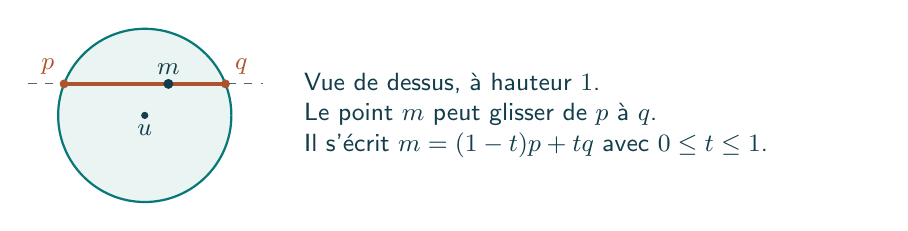
\begin{tikzpicture}[x=1cm,y=1cm,font=\small\sffamily]
\filldraw[draw=accent,fill=wash,thick] (0,0) circle (1.1);
\draw[soft,dashed] (-1.48,.40)--(1.5,.40);
\draw[clay,very thick] (-1.025,.40)--(1.025,.40);
\fill[clay] (-1.025,.40) circle (1.6pt) node[above left] {$p$};
\fill[clay] (1.025,.40) circle (1.6pt) node[above right] {$q$};
\fill[deep] (.3,.4) circle (1.8pt) node[above] {$m$};
\fill[deep] (0,0) circle (1.3pt) node[below] {$u$};
\node[anchor=west,deep,align=left,text width=7.2cm] at (1.9,0)
{Vue de dessus, à hauteur $1$.\\
Le point $m$ peut glisser de $p$ à $q$.\\
Il s'écrit $m=(1-t)p+tq$ avec $0\leq t\leq1$.};
\end{tikzpicture}
\end{center}

\etape{Revenir à la hauteur de départ.}
Pour tout $z\ne0$ dans $W\cap\Om$, de hauteur $s$, le point $z/s$ est sur
ce segment. Il s'écrit $(1-t)p+tq$. On a donc $z=s(1-t)p+stq$, avec deux
coefficients positifs ou nuls. Les vecteurs $p$ et $q$ sont indépendants.
En effet, si $p=kq$, leurs hauteurs égales à $1$ imposeraient $k=1$, donc
$p=q$.

\etape{Séparer les deux directions.} Puisque $p,q$ forment une base de $W$,
on peut écrire de manière unique $T(x)=f(x)p+g(x)q$. En prenant les coordonnées
d'une somme ou d'un multiple, on voit que $f$ et $g$ sont linéaires. Pour
$x\in\Om$, les coefficients $f(x),g(x)$ sont positifs ou nuls d'après la coupe
précédente. Les applications $x\mapsto f(x)p$ et $x\mapsto g(x)q$ préservent
donc le cône. Aucune des deux n'est nulle, sinon $T$ n'aurait qu'une droite
image. Elles sont indépendantes, car leurs droites images sont différentes.

\bilan{Tout élément de $N$ de rang $2$ est la somme de deux éléments indépendants
de $N$. Aucun n'est extrémal.}

\enonce{I.4}{Pourquoi l'identité est-elle extrémale ?}{%
L'endomorphisme identité est-il extrémal ?
}
\etape{Observer l'action sur un vecteur du bord.} L'identité est l'application $\Id(x)=x$. Supposons $\Id=U+V$ avec $U,V\in N$.
Si $p$ est sur le bord, on a $p=U(p)+V(p)$. La propriété du bord force
$U(p)$ à rester sur la demi-droite de $p$. Il reste une difficulté. Le
coefficient pourrait a priori changer quand $p$ change. La linéarité va
l'obliger à prendre la même valeur sur quatre directions bien choisies.

\etape{Comparer les coefficients dans deux directions.} Prenons les quatre vecteurs du bord $u+e_1,u-e_1,u+e_2,u-e_2$. Le premier
couple comme le second a pour somme $2u$. Si $a_i,b_i$ sont les coefficients
de $U$ sur $u+e_i,u-e_i$, on peut donc calculer deux fois le \emph{même}
vecteur $2U(u)$,
\begin{align*}
 2U(u)&=a_1(u+e_1)+b_1(u-e_1)=(a_1+b_1)u+(a_1-b_1)e_1,\\
 2U(u)&=a_2(u+e_2)+b_2(u-e_2)=(a_2+b_2)u+(a_2-b_2)e_2 .
\end{align*}
La deuxième ligne n'a pas de composante suivant $e_1$. Il faut donc $a_1=b_1$.
De même, la première ligne impose $a_2=b_2$. Les composantes suivant $u$
donnent alors $2a_1=2a_2$. Appelons $k$ cette valeur commune des quatre
coefficients. Sur les quatre vecteurs du bord, $U$ multiplie donc par $k$.
Par sommes et différences, cela reste vrai sur $u,e_1,e_2$, puis partout.

\bilan{$U=k\Id$ et $V=(1-k)\Id$ sont dépendants. L'identité est extrémale.}

\enonce{I.5}{Que change la composition par une application envoyant le cône sur lui-même ?}{%
Soit $\alpha$ un endomorphisme de $E$ tel que $\alpha(\Omega)=\Omega$ et soit $\beta$ un endomorphisme extrémal. Les endomorphismes composés $\alpha\circ\beta$ et $\beta\circ\alpha$ sont-ils extrémaux ? l'endomorphisme $\alpha$ est-il extrémal ?
}
\etape{Revenir en arrière avec l'inverse.} L'égalité $\alpha(\Om)=\Om$ signifie que \emph{chaque} vecteur du cône est
atteint. L'image de $\alpha$, qui est un espace vectoriel, contient donc
tout ce que $\Om$ engendre, soit $E$. Le rang vaut $3$. En dimension $3$,
cela rend $\alpha$ inversible. Son inverse $\alpha^{-1}$ ramène aussi $\Om$
sur $\Om$.

\etape{Ramener une décomposition à celle de $\beta$.} Soit $\beta$ extrémal. La notation $\alpha\circ\beta$ indique que l'on applique
$\beta$ puis $\alpha$. Si $\alpha\circ\beta=B+C$ avec $B,C$ indépendants
dans $N$, appliquons $\alpha^{-1}$ après chaque sortie. Il viendrait
\[
                \beta=\alpha^{-1}\circ B+\alpha^{-1}\circ C .
\]
Ces deux termes préservent le cône. Ils restent indépendants, car toute relation
linéaire entre eux redonnerait la même relation entre $B$ et $C$ après application
de $\alpha$. C'est impossible pour $\beta$ extrémal. Pour $\beta\circ\alpha$,
on fait le même calcul en composant à droite par $\alpha^{-1}$.
Enfin, choisir $\beta=\Id$ dans le premier résultat donne $\alpha$ lui-même.

\bilan{$\alpha\circ\beta$, $\beta\circ\alpha$ et $\alpha$ sont tous extrémaux.}

\Needspace{17\baselineskip}
\partie{II}{La famille d’applications}

\enonce{II.1}{Comment annuler la transformation et revenir au vecteur de départ ?}{%
Soit $y$ un élément de $E$ non nul et soit $m=\ps{y}{\sigma(y)}$. Pour tout nombre réel $t$, on désigne par $\alpha_{t,y}$ l'endomorphisme de $E$ tel que
\[
 \alpha_{t,y}(x)=x+\left(\int_0^t e^{m\vartheta}\,d\vartheta\right)
                              \ps{x}{\sigma(y)}y
\]
pour tout $x\in E$. Montrer que, quel que soit $t$, $\alpha_{t,y}$ est de rang $3$ et calculer l'endomorphisme inverse.
}
Le nom $\alpha_{t,y}$ désigne une application qui dépend de deux choix, un nombre $t$ et un vecteur $y$. Fixons $y\ne0$. Dans la formule de l'énoncé, l'intégrale est un \emph{nombre}. L'application part du vecteur $x$ et lui ajoute un multiple de $y$. Pour comprendre ce déplacement, donnons un nom à ses deux coefficients,
\[
 B(x,y)=\ps{x}{\sigma(y)},\qquad m=B(y,y)=q(y),\qquad
 h(t)=\int_0^t e^{m\theta}\,d\theta .
\]
La formule à étudier devient $\alpha_{t,y}(x)=x+h(t)B(x,y)y$. Si $x=su+v$ et $y=au+w$, avec $v,w\perp u$, alors
$B(x,y)=\ps{v}{w}-sa$. On voit que $B(x,y)=B(y,x)$ et que $B$ est \emph{bilinéaire}. Cela signifie que, dans chacun de ses deux arguments, on peut distribuer les sommes et sortir les facteurs numériques.

\etape{Un exemple à calculer à la main.}
Prenons $y=e_1$, un vecteur horizontal de longueur $1$. Alors $\sigma(e_1)=e_1$, $m=1$ et $h(t)=e^t-1$. Pour $x=su+pe_1+re_2$, on a $B(x,e_1)=p$, donc
\[
       \alpha_{t,e_1}(x)=su+e^t p\,e_1+re_2.
\]
Pour $t=-\ln 2$, on a $e^t=1/2$. Le vecteur $3u+2e_1+e_2$ devient $3u+e_1+e_2$. Comment le retrouver ? Il suffit de doubler la coordonnée que l'on vient de diviser par deux. Cela correspond au paramètre opposé, $-t$.

\etape{Retrouver $x$ lorsque $y$ est quelconque.}
Appelons $X=\alpha_{t,y}(x)$ le vecteur d'arrivée. Comme $y$ est connu, il suffit de retrouver le nombre $B(x,y)$ pour soustraire le déplacement ajouté à $x$. Appliquons $B(\,\cdot\,,y)$ à $X$,
\[
 B(X,y)=B(x,y)+h(t)B(x,y)\underbrace{B(y,y)}_{m}
       =(1+mh(t))B(x,y).
\]
Si $m\ne0$, l'intégration donne $h(t)=(e^{mt}-1)/m$. Si $m=0$, on intègre $1$ et $h(t)=t$. Dans les deux cas, $1+mh(t)=e^{mt}>0$. On peut donc diviser et retrouver $B(x,y)=e^{-mt}B(X,y)$. Il vient
\[
 x=X-e^{-mt}h(t)B(X,y)y=X+h(-t)B(X,y)y .
\]
La dernière égalité se lit dans les deux formules de $h$ ci-dessus. Ce calcul donne $\alpha_{-t,y}\circ\alpha_{t,y}=\Id$. Il donne le produit dans l'autre ordre en remplaçant $t$ par $-t$. Toute valeur d'arrivée possède donc un unique antécédent.

\bilan{Pour tout réel $t$, l'inverse est $\alpha_{-t,y}$. L'image est tout $E$, de dimension $3$, donc $\rang(\alpha_{t,y})=3$.}

\enonce{II.2}{Pour quels paramètres l'image reste-t-elle dans le cône ?}{%
Déterminer les valeurs de $t$ pour lesquelles $\alpha_{t,y}\in N$ ainsi que les valeurs de $t$ pour lesquelles $\alpha_{t,y}\in N_+$.
}
Dans l'exemple $y=e_1$, le bord passe par $u+e_1$. Si $e^t=2$, son image est $u+2e_1$, dont l'écart horizontal $2$ dépasse la hauteur $1$. Si $e^t=1/2$, l'application raccourcit au contraire toutes les premières coordonnées horizontales. Voyons pourquoi le signe de $t$ décide aussi dans les autres directions $y$.

\etape{Le calcul qui mesure l'écart au bord.}
Pour un nombre $k$, développons $q(x+ky)=B(x+ky,x+ky)$ comme un carré. La symétrie de $B$ donne
\[
 q(x+ky)=q(x)+2kB(x,y)+k^2q(y).
\]
Ici $k=h(t)B(x,y)$ et $q(y)=m$. Le coefficient de $B(x,y)^2$ devient
$2h(t)+mh(t)^2=h(t)(1+e^{mt})=h(2t)$, d'après les formules de II.1. Ainsi
\[
 \boxed{\ q(\alpha_{t,y}x)=q(x)+h(2t)B(x,y)^2.\ }
\]
Le dernier facteur est un carré. Quant à $h(2t)$, il a le signe de $t$ puisque l’on intègre une fonction positive de $0$ à $2t$, en sens inverse si $t<0$.

\etape{Examiner $t\leq0$.}
Pour $x\in\Om$, $q(x)\leq0$. La formule montre que $q(\alpha_{t,y}x)\leq0$ aussi. Il reste à vérifier la hauteur, car $q\leq0$ décrit à la fois le cône du haut et celui du bas. Si $x\ne0$, faisons varier le paramètre de $0$ à $t$. Les images $\alpha_{r,y}(x)$ forment un trajet continu, commencent en $x$ et sont toutes non nulles par II.1. Pour passer d'une hauteur positive à une hauteur négative, il faudrait atteindre la hauteur $0$. Or à cette hauteur, la condition $q\leq0$ dit $\norm{v}^2\leq0$ et impose le vecteur nul. Le trajet reste donc du côté positif. Pour $x=0$, l'image est simplement $0$.

\etape{Si $t>0$.}
Il suffit de trouver un seul $x\in\Om$ dont l'image sort du cône. Prenons-le sur le bord pour partir de $q(x)=0$. On peut même le choisir parmi les quatre vecteurs $u\pm e_1,\ u\pm e_2$ de sorte que $B(x,y)\ne0$. En effet, si $B(x,y)=\ps{x}{\sigma(y)}$ s'annulait sur les quatre, il s'annulerait sur leurs sommes et différences, donc sur la base $(u,e_1,e_2)$. Cela forcerait $\sigma(y)=0$, puis $y=0$. Pour le $x$ ainsi choisi, la formule encadrée donne $q(\alpha_{t,y}x)>0$.

Enfin $N_+\subset N$. Pour $t=0$, $\alpha_{0,y}=\Id$ est extrémale par I.4. Pour $t<0$, la question suivante donne explicitement les deux termes indépendants qui prouvent l'appartenance à $N_+$.

\bilan{$\alpha_{t,y}\in N$ exactement lorsque $t\leq0$, et $\alpha_{t,y}\in N_+$ exactement lorsque $t<0$.}

\enonce{II.3}{Comment décomposer l'application en termes extrémaux ?}{%
Montrer que si $\alpha_{t,y}\in N$, alors $\alpha_{t,y}$ est somme d'un nombre fini d'endomorphismes extrémaux.
}
Si $t=0$, un seul terme suffit, l'identité. Supposons $t<0$. Nous pouvons utiliser les deux familles déjà connues en I.2 et I.5, à savoir les applications extrémales de rang un et les applications qui envoient le cône sur lui-même.

\etape{Quand $m\ne0$, isolons la direction modifiée.}
Tout $x$ s'écrit $x=p y+z$, où $p=B(x,y)/m$ et $z=x-py$. Ce choix force $B(z,y)=B(x,y)-pm=0$. Dans cette écriture,
\[
       \alpha_{t,y}(py+z)=e^{mt}py+z .
\]
Sur la composante $py$, nous voulons multiplier par $e^{mt}$. Sur $z$, nous voulons multiplier par $1$. Introduisons donc $R(py+z)=-py+z$. Une somme $a\Id+bR$ agit par $a-b$ sur $py$ et par $a+b$ sur $z$. En résolvant $a-b=e^{mt}$ et $a+b=1$, on obtient
\[
      \alpha_{t,y}=\frac{1+e^{mt}}{2}\Id+\frac{1-e^{mt}}{2}R .
\]

\etape{Choisir le signe qui préserve le cône.}
Puisque $B(y,z)=0$, $q(py+z)=p^2m+q(z)=q(-py+z)$. Ainsi $R$ préserve la condition $q\leq0$. De plus, $R^2=\Id$ puisque deux changements de signe successifs s'annulent. Pour savoir où va le haut du cône, testons $u$. Si $y=au+w$, $w\perp u$, on a $B(u,y)=-a$, $m=\norm{w}^2-a^2$ et
\[
 R(u)=u+\tfrac{2a}{m}y,\qquad
 \ps{R(u)}{u}=1+\tfrac{2a^2}{m}=\tfrac{\norm{y}^2}{m}.
\]
Cette hauteur est positive si $m>0$ et négative si $m<0$. Prenons $T=R$ dans le premier cas et $T=-R$ dans le second. Alors $Tu$ a une hauteur positive. Le cône est convexe. En effet, multiplier un de ses vecteurs par un réel positif ou nul préserve son inégalité, et additionner deux de ses vecteurs la préserve aussi par I.2. Les combinaisons $(1-r)x_1+rx_2$ pour $0\leq r\leq1$ restent donc dans le cône. Pour chaque $x\in\Om$ non nul, le segment reliant $u$ à $x$ reste dans le cône avec une hauteur positive. Son image par $T$ reste dans $q\leq0$ et évite $0$ puisque $T^2=\Id$. Elle reste donc du côté de $Tu$, par l'argument de hauteur de II.2. On a $T(\Om)\subset\Om$, puis l'égalité en réappliquant $T$.

Ainsi $T$ est extrémale par I.5. Pour $t<0$, le coefficient $1-e^{mt}$ a le signe de $m$. Notre somme s'écrit donc
\[
      \alpha_{t,y}=\tfrac{1+e^{mt}}2\Id+\tfrac{|1-e^{mt}|}2 T.
\]
Les deux coefficients sont positifs. Les deux termes sont indépendants puisque $R$ change le signe de $y$ et fixe les vecteurs du plan $B(z,y)=0$. Un multiple positif d'une application extrémale reste extrémal, puisqu'on peut toujours diviser une décomposition par ce multiple.

\etape{Quand $m=0$, le vecteur $y$ est sur le bord d'une des deux nappes.}
Remplacer $y$ par $-y$ laisse $B(x,y)y$ inchangé. Choisissons son signe pour avoir $y\in\Om$. Alors $b=-\sigma(y)$ est aussi sur le bord positif, car il garde la hauteur de $y$ et inverse sa partie horizontale. Comme $h(t)=t$, la formule se lit $\alpha_{t,y}(x)=x+(-t)\ps{x}{b}y$. Par I.2, le second terme est extrémal de rang $1$. Il est indépendant de l'identité, qui a rang $3$.

\bilan{Pour $t<0$, on obtient une somme de deux extrémaux indépendants dans les deux cas.}

\enonce{II.4}{Comment trouver un cône intermédiaire qui contient l'ellipse ?}{%
Soit $P$ le plan, ensemble des $x\in E$ tels que $\ps{x}{u}=1$, et soit $S$ une ellipse du plan $P$ contenue dans $\Omega$. Montrer que si $S$ n'est pas le cercle de centre $u$ et de rayon $1$ du plan $P$, alors il existe un $y\in E$, différent de zéro, et un nombre réel $t$ tel que $\alpha_{t,y}\in N_+$ et $S\subset\alpha_{t,y}(\Omega)$.
}
Dans le plan $P$ de hauteur $1$, un point s'écrit $x=u+w$ avec $w$ horizontal. Le disque unité est décrit par $\norm{w}\leq1$. Une ellipse est une courbe obtenue en étirant ou en comprimant un cercle, éventuellement en le déplaçant. Ses demi-axes sont ses deux rayons extrêmes. On nous donne une telle courbe $S$ dans le disque, distincte du cercle qui le borde. On cherche une application $\alpha_{t,y}$ de $N_+$ dont l'image du cône contient toute l'ellipse. Reprenons l'exemple de II.1. Pour $y=e_1$ et $t=-\ln2$, la section de l'image du cône est l'ellipse pleine de demi-axes $1/2$ et $1$.

\begin{center}
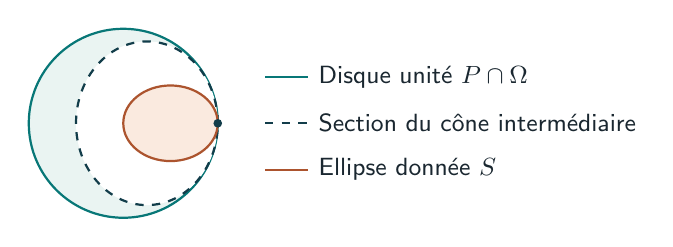
\begin{tikzpicture}[x=1cm,y=1cm,font=\small\sffamily]
\begin{scope}[scale=1.20]
\filldraw[fill=wash,draw=accent,thick] (0,0) circle (1);
\filldraw[fill=white,draw=deep,dashed,thick] (.25,0) ellipse (.75 and .8660254);
\filldraw[fill=peach,draw=clay,thick] (.5,0) ellipse (.5 and .4);
\fill[deep] (1,0) circle (1.3pt);
\end{scope}
\draw[accent,thick] (1.8,.59)--(2.35,.59) node[right,ink] {Disque unité $P\cap\Om$};
\draw[deep,thick,dashed] (1.8,0)--(2.35,0) node[right,ink] {Section du cône intermédiaire};
\draw[clay,thick] (1.8,-.59)--(2.35,-.59) node[right,ink] {Ellipse donnée $S$};
\end{tikzpicture}\par\smallskip
\legende{Un exemple de contact. Les trois contours peuvent passer par le même point.}
\end{center}

\etape{Revenir au cône que nous savons décrire.}
Cherchons $t=-s$ avec $s>0$, car II.2 garantit alors $\alpha_{-s,y}\in N_+$. Par II.1, son inverse est $\alpha_{s,y}$. Dire $x\in\alpha_{-s,y}(\Om)$ revient à dire que $\alpha_{s,y}x\in\Om$. Mesurons la place disponible pour déplacer $x$ en posant
\[
              D(x)=1-\norm{w}^2=-q(x)\quad(x=u+w).
\]
Le nombre $D(x)$ est positif à l'intérieur du disque et nul sur son cercle. Par II.2, la nouvelle valeur de $q$ vaut $-D(x)+h(2s)B(x,y)^2$. Il suffit donc de trouver un $y\ne0$ tel que $B(x,y)^2\leq D(x)$ sur $S$. On prendra ensuite $s$ assez petit pour que $h(2s)\leq1$.

\etape{Traduire le choix de $y$ dans le plan du dessin.}
Une fonction \emph{affine} du point $x=u+w$ a la forme $\ell(x)=a+\ps{b}{w}$, où $a$ est une constante et $b$ un vecteur horizontal. Toutes ces fonctions peuvent servir. En effet, si $y=-au+b$, alors $\sigma(y)=au+b$ et $B(x,y)=a+\ps{b}{w}=\ell(x)$. Une fonction $\ell$ non identiquement nulle donne bien $y\ne0$.

\etape{Si l'ellipse est entièrement à l'intérieur du disque.}
La fonction continue $D$ atteint un minimum $d$ sur l'ellipse, qui est une courbe fermée et bornée. Ici $d>0$, donc la fonction constante $\ell(x)=\sqrt{d}$ convient partout. Si l'ellipse touche le cercle, $d=0$ et il faut construire une fonction qui s'annule aux points de contact. C'est l'objet des deux étapes suivantes.

\etape{Choisir les coordonnées au point de contact.}
On obtient une ellipse en étirant un cercle dans deux directions puis en le déplaçant. Ses points s'écrivent donc
\[
 x=u+c+a\cos\theta+b\sin\theta ,
\]
où $u+c$ est le centre et $a,b$ sont deux vecteurs horizontaux indépendants. On peut faire commencer le parcours en un point de contact, à $\theta=0$. Décaler l'angle revient seulement à remplacer $a,b$ par deux nouvelles combinaisons indépendantes. Écrivons $w_0=c+a$. Le contact donne $\norm{w_0}=1$.

Lorsque $\theta$ varie, $w(\theta)=c+a\cos\theta+b\sin\theta$ reste dans le disque unité. Le carré de sa longueur atteint donc un maximum en $0$. Sa dérivée en $0$ est nulle. Or $w'(0)=b$, d'où $0=2\ps{w_0}{b}$. Géométriquement, au point de contact le mouvement instantané est perpendiculaire au rayon du cercle.

Pour un autre point de l'ellipse, posons $p=\cos\theta-1$ et $r=\sin\theta$. Alors $w=w_0+pa+rb$. Comme $(1+p)^2+r^2=1$, on a $-2p=p^2+r^2$. Tous les termes de la marge se calculent maintenant avec ces deux nombres,
\begin{align*}
 D(x)&=\norm{w_0}^2-\norm{w_0+pa+rb}^2\\
     &=-2p\ps{w_0}{a}-2r\underbrace{\ps{w_0}{b}}_{0}-\norm{pa+rb}^2\\
     &=\ps{w_0}{a}(p^2+r^2)-\norm{pa+rb}^2 .
\end{align*}
Appelons $Q(p,r)$ la dernière expression. En développant le dernier carré, elle a la forme $A p^2+2B_0pr+C r^2$, avec des coefficients réels. Le symbole $B_0$ désigne ici un coefficient numérique.

\etape{Pourquoi $Q$ est-elle positive ou nulle dans toutes les directions ?}
Pour l'instant, nous le savons pour $(p,r)=(\cos\theta-1,\sin\theta)$, car $Q(p,r)=D(x)$. Ces couples sont les vecteurs tracés depuis $(1,0)$ jusqu'aux points du cercle unité dans le \emph{plan des paramètres}. Une droite issue de $(1,0)$ recoupe le cercle, sauf lorsqu'elle est tangente.

Vérifions-le par le calcul. Pour une direction $(d_1,d_2)\ne(0,0)$ avec $d_1\ne0$, le point $(1+\lambda d_1,\lambda d_2)$ est sur le cercle si $2\lambda d_1+\lambda^2(d_1^2+d_2^2)=0$. Il existe bien une solution $\lambda=-2d_1/(d_1^2+d_2^2)\ne0$. Ainsi $Q(\lambda d_1,\lambda d_2)\geq0$. Tous les termes étant de degré deux, il suffit de diviser par $\lambda^2$ pour obtenir $Q(d_1,d_2)\geq0$. La direction $d_1=0$ s'obtient par continuité.

\etape{Extraire le carré d’une fonction affine.}
Nous savons que $Q(p,r)=Ap^2+2B_0pr+Cr^2$ est positive ou nulle pour tous les couples. Elle n'est pas identiquement nulle. En effet, dans ce cas \emph{tous} les points de l'ellipse seraient sur le cercle. Pour vérifier qu'on obtiendrait le cercle entier, appliquons $\norm{c+a\cos\theta+b\sin\theta}=1$ aux angles $0,\pi$ puis $\pi/2,3\pi/2$. En soustrayant les carrés des longueurs de chaque paire, on trouve $c\perp a$ et $c\perp b$. Puisque $a,b$ engendrent le plan horizontal, cela force $c=0$. Les mêmes égalités donnent $\norm{a}=\norm b=1$ et l'angle $\pi/4$ donne $\ps{a}{b}=0$. L'ellipse serait le cercle unité, ce qui est exclu.

En testant $Q$ en $(1,0)$ et $(0,1)$, on voit que $A,C\geq0$. L'un au moins est strictement positif. En effet, s'ils étaient nuls tous deux, les tests en $(1,1)$ et $(1,-1)$ forceraient aussi $B_0=0$. En échangeant les noms $p,r$ dans le calcul si besoin, supposons $A>0$. Complétons un carré,
\[
 Q(p,r)=\left(\sqrt A\,p+\frac{B_0}{\sqrt A}r\right)^2
              +\left(C-\frac{B_0^2}{A}\right)r^2 .
\]
Le second coefficient est positif ou nul, car il vaut $Q(-B_0/A,1)$. La fonction $\ell(x)=\sqrt A\,p+(B_0/\sqrt A)r$ vérifie donc $\ell(x)^2\leq Q(p,r)=D(x)$ sur l'ellipse.

Pourquoi $\ell$ définit-elle une fonction \emph{affine sur le plan} ? Les deux nombres $p,r$ sont précisément les coordonnées de $w-w_0$ dans la base $(a,b)$. On peut donc les calculer pour tout $x=u+w$ du plan, par translation de l'origine en $w_0$ puis lecture des coordonnées. La fonction $\ell$ est non nulle puisque son coefficient devant $p$ vaut $\sqrt A>0$.

\etape{Terminer dans les deux cas, avec ou sans contact.}
Choisissons le vecteur $y\ne0$ correspondant à $\ell$ comme expliqué au début de II.4. Puisque $h(0)=0$ et que $h$ est continue et croissante, on peut choisir $s>0$ tel que $0\leq h(2r)\leq1$ pour tout $0\leq r\leq s$. Pour $x\in S$, la formule de II.2 donne
\[
 q(\alpha_{r,y}x)=-D(x)+h(2r)\ell(x)^2\leq0 .
\]
Comme en II.2, le trajet commence à hauteur $1$ et évite le vecteur nul, donc sa hauteur reste positive. En particulier $\alpha_{s,y}x\in\Om$. En appliquant l'inverse, on obtient $x\in\alpha_{-s,y}(\Om)$ pour chaque $x$ de l'ellipse.

\bilan{Avec ce $y\ne0$ et $t=-s<0$, on a bien $\alpha_{t,y}\in N_+$ et $S\subset\alpha_{t,y}(\Om)$.}

\Needspace{17\baselineskip}
\partie{III}{Classification et décompositions}

\enonce{III.1}{Transmettre une décomposition d'une application à une autre}{%
Soient $\alpha$ et $\beta$ deux endomorphismes de $E$ tels que
\[
                         \beta(\Omega)\subset\alpha(\Omega)\subset\Omega
\]
Montrer que si $\beta$ est de rang $3$ et si $\alpha\in N_+$, alors $\beta\in N_+$.
}
L'inclusion $\beta(\Om)\subset\alpha(\Om)$ dit que toute sortie $\beta(x)$ pour $x\in\Om$ est aussi la sortie de $\alpha$ sur un vecteur du cône.

\etape{Prouver que $\alpha$ est inversible.}
Puisque $\beta$ est de rang $3$, $\beta(E)=E$. Tout vecteur de $E$ est une combinaison linéaire de vecteurs de $\Om$ (I.2). En appliquant $\beta$ à ces combinaisons, on voit que les images des vecteurs de $\Om$ engendrent $E$. Toutes sont dans l'image de $\alpha$, qui est donc $E$ tout entier. Ainsi $\alpha$, de rang $3$ également, est inversible et chaque vecteur possède un unique antécédent.

\etape{Trouver cet antécédent.}
Pour $x\in\Om$, il s'agit de $D(x)=\alpha^{-1}(\beta(x))$. L'inclusion $\beta(\Om)\subset\alpha(\Om)$ garantit que cet antécédent appartient à $\Om$. Donc $D\in N$. De plus, $D$ est inversible car $\alpha$ et $\beta$ le sont. Par construction, $\beta=\alpha\circ D$. Dans cette écriture, \emph{on applique d'abord $D$}, puis $\alpha$.

\etape{Utiliser la décomposition donnée.}
L'hypothèse $\alpha\in N_+$ donne $\alpha=B+C$, où $B,C\in N$ sont indépendants. Pour tout $x$,
\[
   \beta(x)=\alpha(D(x))=B(D(x))+C(D(x)).
\]
Chaque terme envoie $\Om$ dans $\Om$. Vérifions leur indépendance. Si $p(B\circ D)+r(C\circ D)=0$, on a $pB(D(x))+rC(D(x))=0$ pour tout $x$. Or $D(x)$ parcourt tout $E$, puisque $D$ est inversible. Ainsi $pB+rC=0$, ce qui impose $p=r=0$ par indépendance de $B$ et $C$.

\bilan{On a écrit $\beta$ comme somme de deux éléments indépendants de $N$. Donc $\beta\in N_+$.}

\enonce{III.2}{Reconnaître les extrémaux de rang trois}{%
Déterminer les endomorphismes extrémaux de rang $3$ (on utilisera les résultats de II). Le composé de deux endomorphismes extrémaux (de rang quelconque) est-il un endomorphisme extrémal ?
}
Soit $A\in N$ de rang $3$. Nous connaissons déjà des extrémaux de ce rang. Ce sont les applications qui envoient $\Om$ \emph{sur} $\Om$ (I.5). Pour déterminer s'il y en a d'autres, regardons la coupe de $A(\Om)$ à hauteur $1$. Elle nous renseigne sur tout le cône image. En effet, un vecteur du cône de hauteur $h>0$ s'obtient en multipliant par $h$ son point à hauteur $1$.

\etape{Quelle inégalité décrit la coupe ?}
Un point du plan $P$ s'écrit $u+w$, où $w\perp u$. Comme $A$ est inversible, ce point appartient à $A(\Om)$ si son antécédent appartient à $\Om$. Calculons donc
\[
                 F(w)=q\bigl(A^{-1}(u+w)\bigr).
\]
Si $F(w)\leq0$, l'antécédent est dans l'une des deux nappes $\Om$ et $-\Om$. Dans la nappe négative, son opposé serait dans $\Om$. Son image $-(u+w)$ devrait alors être dans $\Om$, alors qu'elle a hauteur $-1$. La nappe positive est donc la seule possible. Réciproquement, un antécédent dans $\Om$ vérifie bien $q\leq0$. La coupe a donc pour équation $F(w)\leq0$.

\etape{Pourquoi cette inégalité dessine-t-elle une ellipse pleine ?}
En coordonnées horizontales $w=re_1+se_2$, $F$ est un polynôme de degré deux, car $A^{-1}$ est linéaire et $q$ est une somme de carrés avec des signes. Les termes de degré deux forment $H(w)=q(A^{-1}w)$. On a $H(w)>0$ pour $w\ne0$. En effet, si $H(w)\leq0$, alors $A^{-1}w$ ou son opposé appartiendrait à $\Om$. Son image $w$ ou $-w$ serait dans $\Om$. C'est impossible pour un vecteur horizontal non nul.

Pour voir le dessin sans supposer ses axes connus, écrivons $H=ar^2+2brs+cs^2$. On a $a>0$ en prenant $(r,s)=(1,0)$. Regroupons les termes en $r$ dans un carré,
\[
 H=a\left(r+\frac ba s\right)^2+d s^2,\qquad d=c-\frac{b^2}{a}>0 .
\]
Le dernier signe se lit en prenant $(r,s)=(-b/a,1)$. Posons $R=r+(b/a)s$. Dans les deux nouvelles coordonnées $R,s$, il ne reste à $F$ que des termes linéaires et une constante en plus de $aR^2+ds^2$. On les absorbe en complétant deux carrés, comme dans $R^2-4R=(R-2)^2-4$. On obtient
\[
                     F=a(R-R_0)^2+d(s-s_0)^2-k .
\]
On a $k>0$ car $F$ prend une valeur négative. En effet, $h=\ps{Au}{u}>0$ et le point $Au/h$ est dans $P$. Son antécédent $u/h$ vérifie $q(u/h)=-1/h^2<0$. Ainsi $F\leq0$ décrit un disque après translation et changement linéaire de coordonnées. En revenant aux coordonnées d'origine, on obtient une ellipse et tout son intérieur. Appelons $S$ son bord.

\etape{Comparer la coupe au disque unité.}
Le grand disque de centre $u$ et de rayon $1$ est la coupe de $\Om$. L'ellipse pleine que nous venons d'obtenir est la coupe de $A(\Om)$. Deux cas sont possibles.

\textbf{1. Les deux coupes coïncident.} En multipliant les points de chaque coupe par toutes les hauteurs possibles, on reconstitue le même cône. Donc $A(\Om)=\Om$. La question I.5 donne l'extrémalité de $A$.

\textbf{2. La coupe de $A(\Om)$ occupe seulement une partie du disque.} Son bord $S$ diffère du cercle unité. C'est précisément le cas étudié en II.4. Cette question fournit une application $T\in N_+$ dont le cône image contient $S$. Il contient également l'intérieur de $S$. En effet, tout point intérieur est situé sur un segment reliant deux points du bord, et $T(\Om)$ contient les segments entre ses points, par convexité. On retrouve alors les inclusions
\[
                       A(\Om)\subset T(\Om)\subset\Om .
\]
Dans III.1, prenons $\beta=A$ et $\alpha=T$. Comme $A$ est de rang $3$, on obtient $A\in N_+$. L'application $A$ admet donc une décomposition en deux éléments indépendants de $N$.

\bilan{Au rang $3$, les extrémaux sont exactement les applications $A$ telles que $A(\Om)=\Om$. On les appelle les \emph{automorphismes du cône}.}

\etape{Que se passe-t-il si l'on compose deux extrémaux ?}
Si l'un des deux est de rang $3$, il est un automorphisme du cône. La question I.5 dit que le composé reste extrémal, quel que soit l'ordre. Si l'un est nul, le composé est nul, donc extrémal au sens de l'énoncé (I.2). Comme le rang $2$ ne donne aucun extrémal, il reste à essayer deux applications de rang $1$.

Écrivons $U(x)=\ps{x}{b}a$ et $V(x)=\ps{x}{d}c$, avec $a,b,c,d$ non nuls sur le bord de $\Om$. Appliquons d'abord $V$, puis $U$. Le nombre $\ps{x}{d}$ sort du produit scalaire. Il vient
\[
           U(V(x))=\ps{\ps{x}{d}c}{b}a
                    =\ps{c}{b}\ps{x}{d}a.
\]
Par I.1, $\ps{c}{b}\geq0$. S'il est positif, il multiplie le vecteur $a$ par un nombre positif, ce qui laisse ce vecteur sur le bord. Le composé est donc extrémal de rang $1$ par I.2. S'il est nul, le composé est nul. Cela peut arriver, par exemple avec $b=u+e_1$ et $c=u-e_1$, dont le produit scalaire vaut $1-1=0$.

\bilan{Oui. Le composé de deux extrémaux est toujours extrémal, même si son rang peut diminuer.}

\enonce{III.3}{Peut-on tout construire par additions d'extrémaux ?}{%
Tout endomorphisme de $E$ appartenant à $N$ est-il la somme d'un nombre fini d'endomorphismes extrémaux ? (on pourra commencer par étudier le cas d'un endomorphisme $\alpha\in N$ de rang $3$ tel que l'intersection de $\alpha(\Omega)$ et du plan $P$ défini en II-4) soit un cercle et son intérieur ; on montrera que, dans ce cas, il existe un $z\in\Omega$ tel que $\alpha(\Omega)$ soit l'image de $\Omega$ par l'endomorphisme qui transforme tout $x\in E$ en $x+\ps{x}{u}z$).
}
\etape{Un exemple pour comprendre l'indication.}
Partons du disque unité à hauteur $1$. L'application $x\mapsto x+\ps{x}{u}u$ envoie $u+v$ sur $2u+v$. Ce résultat est à hauteur $2$. Quand on le divise par $2$ pour le ramener à hauteur $1$, on trouve $u+v/2$. La coupe du cône image est donc un disque de rayon $1/2$. On peut aussi déplacer le centre de ce disque en ajoutant une composante horizontale.

\etape{Le disque de centre et de rayon donnés.}
Supposons, comme dans l'indication, que $A$ soit de rang $3$ et que la coupe de $A(\Om)$ soit un disque de centre $u+c$ et de rayon $r>0$, avec $c\perp u$. Ce disque tient dans le disque unité. Son point le plus éloigné de $u$ est à distance $\norm c+r$, donc $\norm c+r\leq1$.

Nous cherchons $L_z(x)=x+\ps{x}{u}z$. Sur le disque unité, $L_z$ ajoute simplement $z$ puisque $\ps{x}{u}=1$. Nous voulons que $u+v$ devienne $u+c+rv$ après retour à hauteur $1$. Il suffit donc d'obtenir, \emph{avant} cette division, $u/r+c/r+v$. Cela donne le choix
\[
  z=\left(\frac1r-1\right)u+\frac cr,\qquad
  L_z(u+v)=\frac1r(u+c+rv).
\]
La hauteur de $z$ est $(1-r)/r$ et sa longueur horizontale est $\norm c/r$. L'inégalité $\norm c+r\leq1$ garantit que $z\in\Om$. Les coupes de $L_z(\Om)$ et de $A(\Om)$ sont bien le même disque. Ainsi $L_z(\Om)=A(\Om)$.

\etape{En déduire une somme dans ce cas.}
L'application $L_z$ est inversible puisque son image contient $A(\Om)$, qui engendre $E$. Posons $C=L_z^{-1}\circ A$. L'égalité des cônes images donne $C(\Om)=\Om$. On a $A=L_z\circ C$, et composer avec $C$ conserve l'extrémalité par I.5. Il suffit donc de décomposer $L_z$.

L'identité est déjà extrémale. Il reste, dans $L_z(x)=x+\ps{x}{u}z$, à décomposer le terme $\ps{x}{u}z$. Tout vecteur $p=hu+v\in\Om$ est somme d'au plus deux vecteurs du bord. En prenant $e=v/\norm v$ pour $v\ne0$ et un vecteur horizontal unitaire quelconque sinon, on vérifie
\[
  p=\frac{h+\norm v}{2}(u+e)+\frac{h-\norm v}{2}(u-e).
\]
Les coefficients sont positifs ou nuls car $h\geq\norm v$. Écrivons ainsi $u=u_1+u_2$ et $z=z_1+z_2$. En développant $\ps{x}{u_1+u_2}(z_1+z_2)$, on obtient au plus quatre termes non nuls $\ps{x}{u_i}z_j$. Chacun est extrémal de rang $1$ par I.2. Cela résout le cas du disque.

\etape{Le cas général. Pourquoi faut-il une autre idée ?}
Par définition, une application non extrémale se partage en deux. Mais si on choisit les deux morceaux au hasard, rien ne garantit que les partages suivants s'arrêtent. Nous allons choisir les morceaux \emph{aux extrémités d'un segment}. À chaque extrémité, on perdra au moins une direction dans laquelle on pouvait encore bouger.

\etape{Comparer des applications à la même échelle.}
Pour $T\in N$, prenons la hauteur $\eta(T)=\ps{Tu}{u}$. Elle est positive ou nulle car $Tu\in\Om$. Elle ne peut être nulle que pour $T=0$. En effet, la hauteur nulle donnerait $Tu=0$. Pour $i=1,2$, les deux vecteurs $T(u+e_i)$ et $T(u-e_i)$ seraient dans $\Om$ et leur somme serait $2Tu=0$. Le cône ne contient pas de vecteurs opposés non nuls. Toutes ces images seraient donc nulles, et les $u\pm e_i$ engendrent $E$.

On peut donc diviser chaque $T\ne0$ par sa hauteur et travailler dans l'ensemble
\[
                     K=\{T\in N:\eta(T)=1\}.
\]
On rétablira le facteur $\eta(T)$ à la fin. Dans $K$, une application est extrémale exactement lorsqu'elle n'est \emph{entre} deux éléments distincts de $K$ sur aucun segment. Voyons pourquoi. Si $T=B+C$ avec $B,C\in N$ indépendants, posons $p=\eta(B)$ et $r=\eta(C)$. On a $p,r>0$, $p+r=1$ et
\[
                       T=p(B/p)+r(C/r).
\]
C'est une moyenne pondérée de deux éléments distincts de $K$. Réciproquement, une telle moyenne donne deux termes indépendants dans $N$. En effet, deux éléments proportionnels de $K$ sont égaux, puisque leur hauteur vaut $1$.

\etape{Pourquoi rencontre-t-on une extrémité ?}
L'ensemble $K$ contient tous les segments entre ses points, car les moyennes pondérées conservent le cône et la hauteur $1$. Il est fermé. En effet, si les coefficients de matrices dans $K$ convergent, leurs images de chaque $x\in\Om$ restent dans $\Om$ à la limite, car la condition $h\geq\norm v$ est une inégalité large. La hauteur de $Tu$ reste $1$ à la limite aussi.

Enfin, les coefficients des matrices de $K$ sont bornés. Pour le voir, $T(u+e_i)$ et $T(u-e_i)$ sont dans $\Om$ et leurs hauteurs ont pour somme $2\eta(T)=2$. Chaque hauteur est donc entre $0$ et $2$. Dans le cône, la longueur horizontale est au plus la hauteur, donc chaque coordonnée de ces images a valeur absolue au plus $2$. Leurs demi-sommes et demi-différences donnent $Tu$ et $Te_i$. Cela borne toutes les colonnes de la matrice de $T$.

Si l'on bouge sur une droite $T+sH$ avec $H\ne0$, au moins un coefficient de la matrice change à vitesse non nulle. Il finirait donc par dépasser ces bornes si $|s|$ devenait trop grand. Sur une telle droite, la partie autorisée forme donc un segment fermé dès qu'elle contient plusieurs points.

\etape{Choisir les deux morceaux et prouver l'arrêt.}
Voici la figure obtenue sur une droite passant par $T$, lorsqu'on peut bouger à partir de $T$ dans les deux sens. Chaque point du dessin représente une \emph{application}.

\begin{center}
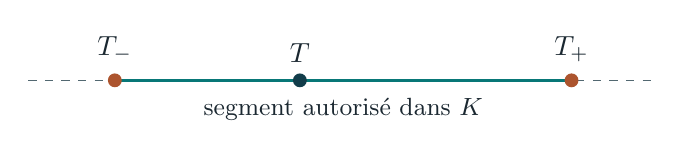
\begin{tikzpicture}[x=1cm,y=1cm]
\draw[thin,soft,dashed] (-4,0)--(4,0);
\draw[accent,very thick] (-2.9,0)--(2.9,0);
\fill[clay] (-2.9,0) circle (2.5pt) node[above=3pt,ink] {$T_-$};
\fill[deep] (-.55,0) circle (2.5pt) node[above=3pt,ink] {$T$};
\fill[clay] (2.9,0) circle (2.5pt) node[above=3pt,ink] {$T_+$};
\node[below=3pt,ink,font=\small] at (0,0) {segment autorisé dans $K$};
\end{tikzpicture}
\end{center}

Comptons les directions disponibles. Écrivons $V(T)$ pour l'ensemble des applications $H$ pour lesquelles $T+\varepsilon H$ et $T-\varepsilon H$ restent dans $K$ pour un $\varepsilon>0$. Ce sont exactement les directions dans lesquelles un petit déplacement est possible \emph{des deux côtés}.

Ces directions forment un espace vectoriel. Multiplier $H$ par un nombre change seulement la longueur du petit pas à choisir. Pour additionner $H_1$ et $H_2$, choisissons $\varepsilon$ assez petit pour que $T\pm2\varepsilon H_1$ et $T\pm2\varepsilon H_2$ soient dans $K$. Les moyennes des deux points avec le même signe donnent $T\pm\varepsilon(H_1+H_2)\in K$. On peut donc bien compter le nombre de directions indépendantes. C'est la dimension de $V(T)$.

Si ce nombre vaut zéro, $T$ est extrémal, d'après le critère du segment établi ci-dessus. Sinon, choisissons $H\ne0$ dans $V(T)$. Allongeons le segment sur la droite $T+sH$ jusqu'à ses deux extrémités $T_-$ et $T_+$. Puisque $T$ est entre elles, il existe $0<p<1$ tel que $T=pT_-+(1-p)T_+$.

Voici pourquoi on a progressé. Une direction $G$ possible en $T_-$ est aussi possible en $T$. Dans la moyenne ci-dessus, remplaçons $T_-$ par $T_-\pm\varepsilon G$ en gardant $T_+$ fixe. Les résultats $T\pm p\varepsilon G$ sont encore dans $K$. Donc $V(T_-)\subset V(T)$. En revanche, $H$ appartient à $V(T)$ et ne peut plus appartenir à $V(T_-)$, puisqu'on sortirait du segment en continuant au-delà de cette extrémité. L'inclusion est donc stricte. Il en va de même pour $T_+$.

À chaque partage, \emph{chacun} des deux morceaux a donc strictement moins de directions disponibles. Au départ leur nombre est au plus $9$, car une application de $E$ dans $E$ est décrite par une matrice à neuf coefficients. Après au plus neuf partages successifs le long d'une branche, il reste zéro direction. Il n'y a que deux morceaux par partage. On aboutit donc à une moyenne pondérée \emph{finie} d'extrémaux.

\bilan{Oui. On rétablit la hauteur initiale et on incorpore chaque coefficient positif à son extrémal. Un multiple positif d'un extrémal reste extrémal. L'application nulle est déjà extrémale d'après I.2.}

\enonce{III.4}{Peut-on imposer le rang un à tous les termes ?}{%
L'endomorphisme $\gamma$ de $E$ défini par $\gamma(x)=-x+\frac{5}{2}\ps{x}{u}u$ est-il la somme d'un nombre fini d'endomorphismes extrémaux de rang $1$ ?
}
Cette fois, l'application à décomposer est $\gamma(x)=-x+\tfrac52\ps{x}{u}u$. Pour exclure une décomposition de rang $1$, cherchons un nombre qui s'additionne quand on additionne les applications. Si ce nombre est positif ou nul pour tous les morceaux, leur somme ne pourra jamais lui donner une valeur négative.

\etape{Le nombre choisi est la trace.}
La trace d'une matrice est la somme des nombres de sa diagonale, du coin supérieur gauche au coin inférieur droit. Par exemple, une diagonale $(2,0,3)$ donne une trace $2+0+3=5$. Dans un repère fixé, additionner deux matrices consiste à additionner les nombres case par case. Les traces s'additionnent donc aussi.

Pour un élément de $N$ de rang $1$, on a $T(x)=\ps{x}{b}a$ avec $a,b\in\Om$. Dans une base orthonormée, notons $a_i,b_i$ leurs coordonnées. La colonne numéro $j$ donne l'image du $j$-ième vecteur de base, c'est-à-dire $b_j a$. Le coefficient situé sur la diagonale dans cette colonne vaut donc $b_j a_j$. Ainsi
\[
        \tr(T)=a_1b_1+a_2b_2+a_3b_3=\ps{a}{b}\geq0 .
\]
L'inégalité vient de I.1 puisque $a$ et $b$ sont dans $\Om$.

\etape{Calculer cette même quantité pour $\gamma$.}
Prenons le repère $(e_1,e_2,u)$. Pour $e_1$ et $e_2$, le produit scalaire avec $u$ vaut $0$. Leurs images sont donc $-e_1$ et $-e_2$. Pour $u$, ce produit vaut $1$ et l'image est $-u+\tfrac52u=\tfrac32u$. Les colonnes sont maintenant connues,
\[
    [\gamma]=\begin{pmatrix}-1&0&0\\0&-1&0\\0&0&3/2\end{pmatrix},
    \qquad \tr(\gamma)=-1-1+\tfrac32=-\tfrac12 .
\]
\bilan{Non. Une somme d'extrémaux de rang $1$ aurait une trace positive ou nulle. La trace de $\gamma$ vaut $-1/2$.}

\smallskip

\label{fin}

\end{document}